Particle accelerators were first developed in the early 20th century as a tool for high-energy physics research. By increasing particles' energy they allow us to investigate the subatomic structure of the world and to study the properties of the elementary particles and the fundamental forces. On a basic level, accelerators increase the energy of charged particles using electromagnetic fields. Through the years significant technological progress has been achieved resulting in higher energies and optimising the performance of the machines. Additionally, various types of accelerators have been developed (synchrotrons, colliders etc) using different types of particles (hadrons or leptons) and its use was also expanded in other fields such as medicine and industrial research. 
% Brief history of particle accelerators: https://cds.cern.ch/record/261062/files/p1_2.pdf
% Summary for accelerators: https://www.energy.gov/articles/how-particle-accelerators-work#:~:text=There%20are%20two%20primary%20roles,charged%20particles%20for%20medical%20treatment.



\section{The CERN accelerator complex}

CERN (European Organisation of Nuclear Research), located on the Franco-Swiss border near Geneva, is at the forefront of the accelerator physics research as it operates an extensive network of accelerators, illustrated in Fig.~\ref{fig:cern_accelerator_complex}, including the well-known Large Hadron Collider (LHC)~\cite{Brüning:782076}.

LHC is a circular machine, 27\, km long, built about 100\,m underground and is currently the largest and most powerful accelerator. It accelerates and collides two counter-rotating beams at the four main experiments which are located around the LHC ring, namely ATLAS, CMS, ALICE and LHCb. The highlight of CERN and of the LHC operation up to now was the discovery of the Higgs boson in 2012 from ATLAS~\cite{ATLAS_Higgs} and CMS~\cite{CMS_Higgs}, from proton collisions at a total energy of 7\,TeV, which was a milestone for the standard model. % Importance of higgs discovery: https://home.cern/resources/faqs/cern-and-higgs-boson


LHC is taking the beam from the injectors which operate in a chain poviding increasingly higher energy to the beam. In particular, Linas, psd, ps sps.


Not only protons but heavy ions. 
and a number of smaller accelerators and deccelerators like AD, isolde etc.




\begin{figure}[!h] %https://cds.cern.ch/images/CERN-GRAPHICS-2022-001-1
    \centering         
    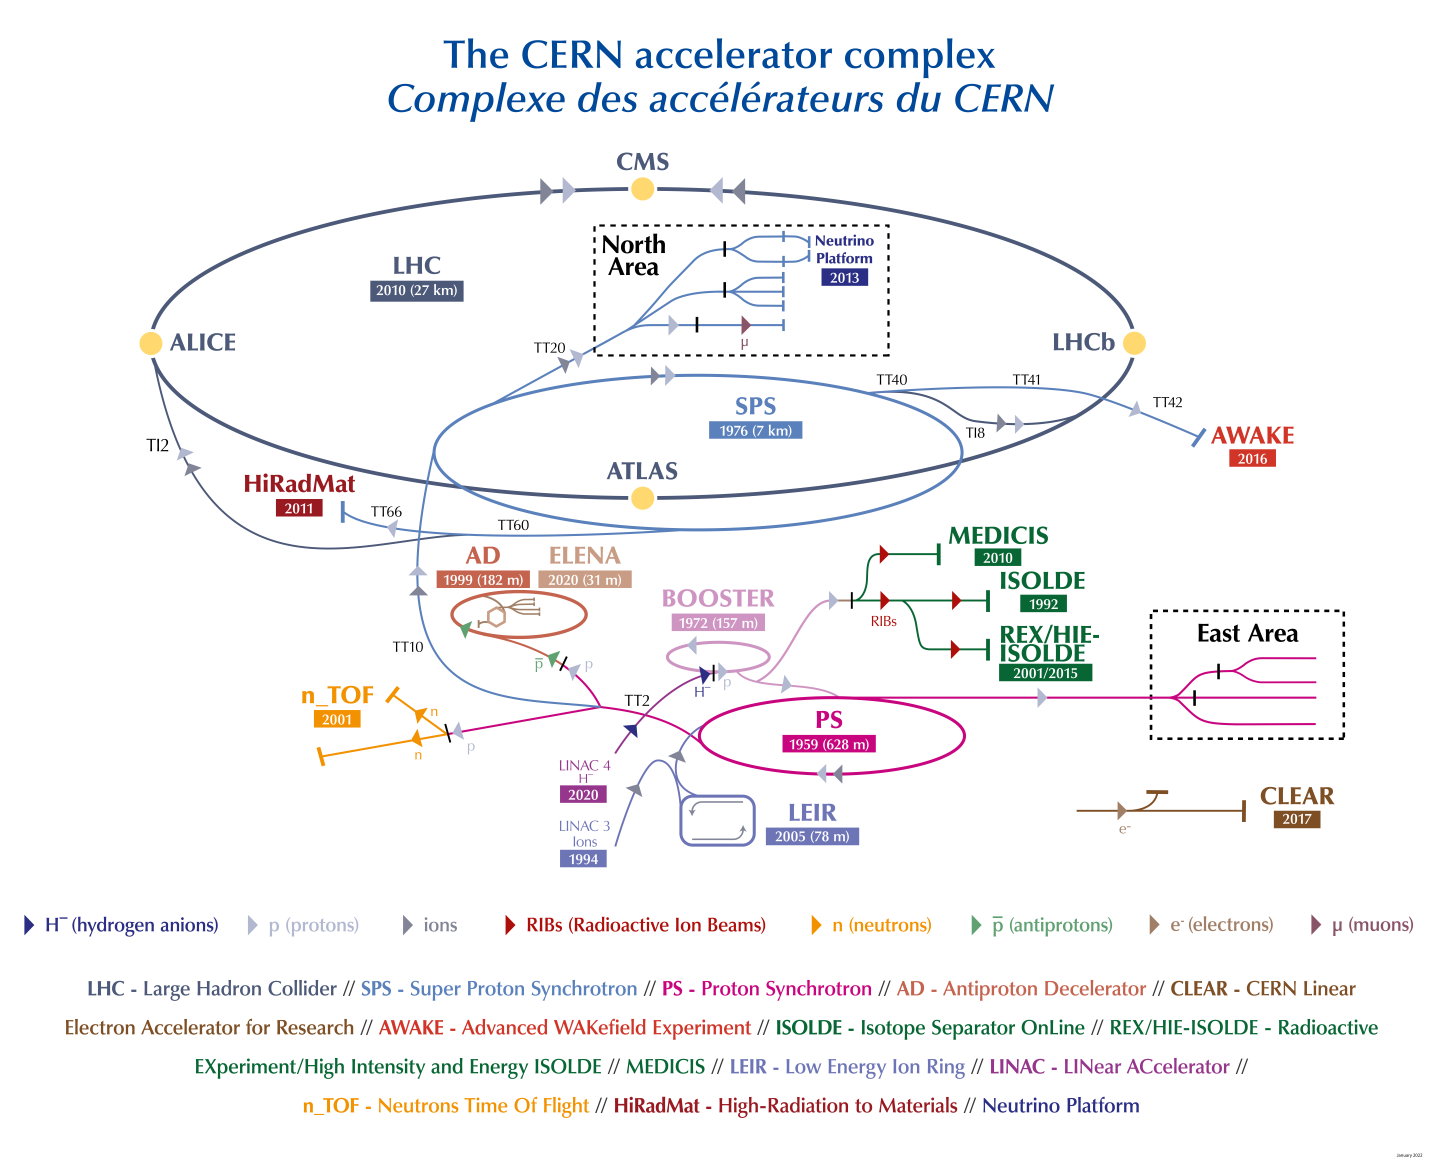
\includegraphics[width=1\textwidth]{images/introduction/cern_accelerator_complex.png}
        \caption{Schematic view of the CERN accelerator complex. The different colors correspond to the different machines. The year of commissioning and the type of particles used in each one of them are also indicated along with the circumference for the circular machines. The image is a courtesy of CERN.}
        \label{fig:cern_accelerator_complex}
 \end{figure}


 LHC is the latest addition (2010) in the CERN accelerator complex which consists of eight accelerators and two decelerators. 

 grapse gia to acclerator cmplez
 not only protons 
fixed target experiments
decelerators.




The studies in this thesis, will focus on LHC and the SPS. and for proton collisions.


\subsection{The Super Proton Synchrotron - SPS}





\newpage
1. General about standard model (Sofia, Schenk)
2. Role of CERN
3. Role of my thesis.


\section{High-Luminosity LHC project and Crab Cavities}
continuous importvements for energy and luminosity.

For hl-lhc:

https://hilumilhc.web.cern.ch/

Why do we need hl-lhc.
%https://slideplayer.com/slide/8611970/ slide 3

extend/push the discovery potential (Sofia.)

HL-lHC a major upgrade, priority of the european strategy





High-Luminosity LHC (HL-LHC) project~\cite{HL-LHC} is the upgrade of the LHC machine, which aims to increase its integrated luminosity production by a factor of 10 beyond the current operational values.


Crab cavities (will be denoted as $\CC$ in this thesis) is one of the key components of the High Luminosity LHC


\section{Motivation, objectives and thesis outline}

\textbf{Probably put to abstract}\\
In 2018, two prototype Crab Cavities ($\CC$s) were installed in the SPS to be tested for the first time with proton beams. A series of dedicated machine developemnt studies was carried out in order to validate their working principle and answer various beam dynamic questions. One of the operational issues that needed to be addressed concerned the expected emittance growth due to noise in their RF system, which is the main subject this thesis.  As mentioned in chapter~\ref{Ch:CC_noise_theory} a theoretical model had already been developed and validated by trackig simulations~\cite{PhysRevSTAB.18.101001}. 
As a part of the first experiemental campaign with $\CC$s in SPS a dedicated experiment was conducted to benchmark these models with experimental data and confirm the analytical predictions. The objective of this chapter is to provide an overview of the machine setup for the $\CC$ experiements and introduce the instruments and methods used for measuring the beam parameters of interest for the emittance growth studies.

\section{General parameters of the studies}
% Maybe this should be mentioned at the end of project objectives and thesis outline.
% The following paragraphs are taken from the APR Ch.1.3 
\subsection{SPS optics}\label{subsec:SPS_optics_model}
 The studies presented in this thesis were performed for the nominal SPS optics for the LHC filling which are called Q26 optics as the higher integer part of the tune in both planes is 26. 

 \normalsize{\textbf{SPS nominal model}\\
 The model for the Q26 optics can be found in the official CERN repository~\cite{SPS_optics_repo} and will be referred to as the nominal SPS model in this thesis. The values of the optics parameters in what follows correspond to the model values unless stated otherwise.

 \normalsize{\textbf{SPS non-linear model}\\
The nominal SPS model includes only the nonlinear fields produced by the chromatic sextupoles. However, one of the most important sources of non-linearities in SPS are the odd multipole components of its main dipole magnets. For some of the studies presented in this thesis their impact on the beam dynamics must be studied and therefore they should be included in the nominal model. 

% APR Chapter 3.1
The multipole error of the SPS main dipoles are unfortunately not available from magnetic measurements. On this ground a non-linear optics model of the SPS has been established with beam-based measurements of the chromatic detuning over a range of momentum deviation~\cite{Carlà:2664976, Alekou:2640326}.  The optics model was obtained by assigning systematic multipole components to the main lattice magnets, in the nominal model of SPS, in order to reproduce the tune variation with themomentum deviation as it was measured in the real machine. The calculations were performed with MAD-X [].

The values of the multipole components up to seventh order obtained from this method are given in Table~\ref{tab:sps_mult_270GeV} where, ($b_3^A, b_3^B$) ($b_5^A, b_5^B$) and ($b_7^A, b_7^B$) stand for the sextupolar, decapolar and decatetrapolar mutipoles respectively. Note that different values have been obtained foreach of the two different kinds of SPS main dipoles (MBA and MBB) which are marked withthe indices A and B respectively.

\begin{table}[ht] % table take from the APR
    \caption{Multipole errors from SPS non-linear model, at 270\,GeV.} % title of Table
    \centering % used for centering table
    \begin{tabular}{c c c c} % centered columns (4 columns)
    \hline\hline %inserts double horizontal lines
    Multipole & Value  \\ [0.5ex] % inserts table
    %heading
    \hline  % inserts single horizontal line
    $b_3^A, b_3^B$ & 8.1 $\times 10^{-4}$\,$\mathrm{m^{-2}}$, 1.1 $\times 10^{-3}$\,$\mathrm{m^{-2}}$\\ 
    $b_5^A, b_5^B$ & 9.2\,$\mathrm{m^{-4}}$, $-$10\,$\mathrm{m^{-4}}$ \\
    $b_7^A, b_7^B$ & 1.3 $\times 10^{5}$\,$\mathrm{m^{-6}}$, 1.4 $\times 10^{5}$\,$\mathrm{m^{-6}}$\\ [1ex] % [1ex] adds vertical space
    \hline %inserts single line
    \end{tabular}
    \label{tab:sps_mult_270GeV} % is used to refer this table in the text
    \end{table}


\textbf{random multiple errros? } Like in APR.Ch.3.2.2.